\documentclass[12pt,a4paper]{article}
\usepackage{huy}
\begin{document}
\intro{\db}{Subqueries}
\section{Subqueries}
A subquery is a query that is nested inside a SELECT, INSERT, UPDATE, or DELETE statement, or inside another subquery. A subquery can be used anywhere an expression is allowed. A subquery is also called an inner query or inner select, while the statement containing a subquery is also called an outer query or outer select. The following shows an example of subqueries:
\begin{lstlisting}[language=SQL,style=cool]
SELECT Name
FROM AdventureWorks2008R2.Production.Product
WHERE ListPrice =
    (SELECT ListPrice
     FROM AdventureWorks2008R2.Production.Product
     WHERE Name = 'Chainring Bolts' );
\end{lstlisting}
Many Transact-SQL statements that include subqueries can be alternatively formulated as joins. The following is an example showing a join SELECT that return the same result set as the previous example:
\begin{lstlisting}[language=SQL,style=cool]
SELECT Prd1. Name
FROM AdventureWorks2008R2.Production.Product AS Prd1
     JOIN AdventureWorks2008R2.Production.Product AS Prd2
       ON (Prd1.ListPrice = Prd2.ListPrice)
WHERE Prd2. Name = 'Chainring Bolts';
\end{lstlisting}
The SELECT query of a subquery is always enclosed in parentheses. A subquery can be nested inside the WHERE or HAVING clause of an outer SELECT, INSERT, UPDATE, or DELETE statement, or inside another subquery. A subquery can appear anywhere an expression can be used, if it returns a single value. If a table appears only in a subquery and not in the outer query, then columns from that table cannot be included in the output (the select list of the outer query).
\section{Practical part}
Find the branch where Ann works. Include at least columns Street and City
from Branch table. If you want to include column FirstName from Staff table,
you need to use JOIN operation.
\database{1-Ann-branch.sql}
\begin{figure}[hbtp]
	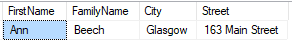
\includegraphics[scale=1]{1-Ann-branch.PNG}
	\end{figure}
List the Staff who work in the branch at ’32 Manse Road’… and only those
whose position is ‘Assistant’ in that same branch. Include at least columns
FirstName and FamilyName from Staff table. If you want to include column
Street information from Branch table, you need to use JOIN operation.
\database{2-branch-position.sql}
\begin{figure}[hbtp]
	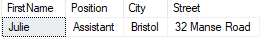
\includegraphics[scale=1]{2-branch-position.PNG}
	\end{figure}
Find the owner of the property for rent at address ‘Slippery Lane 16’.
Include at least columns FirstName and FamilyName from PrivateOwner
table. If you want to include column Street information from PropertyForRent
table, you need to use JOIN operation.
\database{3-owner-street.sql}
\begin{figure}[hbtp]
	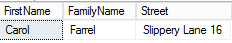
\includegraphics[scale=1]{3-owner-street.PNG}
	\end{figure}
List the names of all clients who have viewed a property at 15th of June.
Include at least columns FirstName and FamilyName from Client table. If you
want to include column ViewDate information from Viewing table, you need to
use JOIN operation. Using JOIN needs also keyword DISTINCT.
\database{4-viewdate.sql}
\begin{figure}[hbtp]
	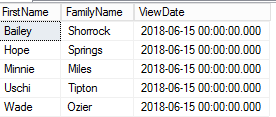
\includegraphics[scale=1]{4-viewdate.PNG}
	\end{figure}
List the names of all clients who have viewed a property at 15th of June or
at 16th of June. Include at least columns FirstName and FamilyName from
Client table. If you want to include column ViewDate information from Viewing
table, you need to use JOIN.
\database{5-2viewdate.sql}
\begin{figure}[hbtp]
	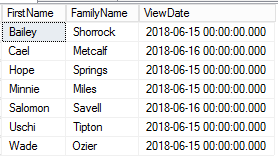
\includegraphics[scale=1]{5-2viewdate.PNG}
	\end{figure}
List the name of all clients who has viewed a property at 15th of June and
who did not give any comments. Include at least columns FirstName and
FamilyName from Client table.
\database{6-null-comment.sql}
\begin{figure}[hbtp]
	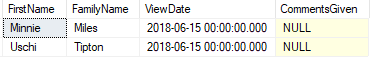
\includegraphics[scale=1]{6-null-comment.PNG}
	\end{figure}
Find the name of a staff member who manages property for rent at ‘8
Naval Drive’. Include at least columns FirstName and FamilyName from Staff
table.
\database{7-staff-street.sql}
\begin{figure}[hbtp]
	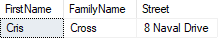
\includegraphics[scale=1]{7-staff-street.PNG}
	\end{figure}
Find the names of all clients who have viewed Flats. Include at least
columns FirstName and FamilyName from Client table. 
\database{8-view-flat.sql}
\begin{figure}[hbtp]
	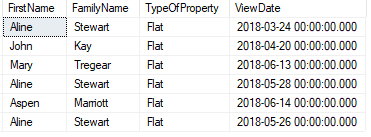
\includegraphics[scale=1]{8-view-flat.PNG}
	\end{figure}
\end{document}